
% ----------------------------------------------------------------------
% Set the document class
% ----------------------------------------------------------------------
\documentclass[12pt]{article}
\usepackage{multirow}
\usepackage{matlab-prettifier}



% ----------------------------------------------------------------------
% Define external packages, language, margins, fonts, new commands 
% and colors
% ----------------------------------------------------------------------
\usepackage[utf8]{inputenc} % Codification
\usepackage[english]{babel} % Writing idiom

\usepackage[export]{adjustbox} % Align images
\usepackage{amsmath} % Extra commands for math mode
\usepackage{amssymb} % Mathematical symbols
\usepackage{anysize} % Personalize margins
    \marginsize{2cm}{2cm}{2cm}{2cm} % {left}{right}{above}{below}
\usepackage{appendix} % Appendices
\usepackage{cancel} % Expression cancellation
\usepackage{caption} % Captions
    \DeclareCaptionFont{newfont}{\fontfamily{cmss}\selectfont}
    \captionsetup{labelfont={bf, newfont}}
\usepackage{cite} % Citations, like [1 - 3]
\usepackage{color} % Text coloring
\usepackage{fancyhdr} % Head note and footnote
    \pagestyle{fancy}
    \fancyhf{}
    \fancyhead[L]{\footnotesize \fontfamily{cmss}\selectfont Embedded Systems} % Left of Head note
    \fancyhead[R]{\footnotesize \fontfamily{cmss}\selectfont CE5439} % Right of Head note
    \fancyfoot[L]{\footnotesize \fontfamily{cmss}\selectfont CE Dep.} % Left of Footnote
    \fancyfoot[C]{\thepage} % Center of Footnote
    \fancyfoot[R]{\footnotesize \fontfamily{cmss}\selectfont AUT} % Right of Footnote
    \renewcommand{\footrulewidth}{0.4pt} % Footnote rule
\usepackage{float} % Utilization of [H] in figures
\usepackage{graphicx} % Figures in LaTeX
\usepackage[colorlinks = true, plainpages = true, linkcolor = blue, urlcolor = blue, citecolor = blue, anchorcolor = blue]{hyperref}
\usepackage{indentfirst} % First paragraph
\usepackage[super]{nth} % Superscripts
\usepackage{siunitx} % SI units
\usepackage{subcaption} % Subfigures
\usepackage{titlesec} % Font
    \titleformat{\section}{\fontfamily{cmss}\selectfont\Large\bfseries}{\thesection}{1em}{}
    \titleformat{\subsection}{\fontfamily{cmss}\selectfont\large\bfseries}{\thesubsection}{1em}{}
    \titleformat{\subsubsection}{\fontfamily{cmss}\selectfont\normalsize\bfseries}{\thesubsubsection}{1em}{}
    \fancyfoot[C]{\fontfamily{cmss}\selectfont\thepage}

% Random text (not needed)
\usepackage{lipsum}
\usepackage{duckuments}

% New and re-newcommands
\newcommand{\sen}{\operatorname{\sen}} % Sine function definition
\newcommand{\HRule}{\rule{\linewidth}{0.5mm}} % Specific rule definition
\renewcommand{\appendixpagename}{\LARGE \fontfamily{cmss}\selectfont Appendices}

% Colors
\definecolor{istblue}{RGB}{3, 171, 230}
\definecolor{dkgreen}{rgb}{0,0.6,0}
\definecolor{gray}{rgb}{0.5,0.5,0.5}

% Image path
\graphicspath{ {./Images/} }
%%%%%%%%%%%%%%%%%%%%%%%%%%%%%%%%%%%%%%%%%%%%%%%%%%%%%%%%%%%%%%%%%%%%%%%%
%                                 Document                             %
%%%%%%%%%%%%%%%%%%%%%%%%%%%%%%%%%%%%%%%%%%%%%%%%%%%%%%%%%%%%%%%%%%%%%%%%
\begin{document}

% ----------------------------------------------------------------------
% Cover
% ----------------------------------------------------------------------
\begin{center}
    \begin{figure}
        \vspace{-1.0cm}
        \centering
        
\includegraphics[scale = 0.35]{Images/AUT_logo.png} % IST logo
    \end{figure}
    \mbox{}\\[2.0cm]
    \textsc{\Huge \textbf{Embedded Systems Modeling and Design}}\\[1.0cm]
    \textsc{\LARGE Instructor: \href{https://scholar.google.com/citations?user=2RN0Y2YAAAAJ&hl=en}{\textcolor{black}{Prof. Mehdi Sedighi}}}\\[2.5cm]
    \textsc{\LARGE Amirkabir University of Technology} \\%\\[1.0cm]
    \textsc{(Tehran polytechnic)}
    \HRule\\[0.4cm]
    {\large \bf {\fontfamily{cmss}\selectfont Design and Modeling of an Intelligent Automotive Airbag System \& Petri Net-Based Modeling of an Elevator System} }\\[0.2cm]
    \HRule\\[1.5cm]
\end{center}

\begin{flushleft}
    \textbf{\fontfamily{cmss}\selectfont Authors:}
\end{flushleft}

\begin{center}
    \begin{minipage}{0.5\textwidth}
        \begin{flushleft}
            \href{https://rezaadinepour.github.io/}{\textcolor{black}{Reza Adinepour}}\\
        \end{flushleft}
    \end{minipage}%
    \begin{minipage}{0.5\textwidth}
        \begin{flushright}
            \href{mailto:adinepour@aut.ac.ir}{\texttt{adinepour@aut.ac.ir}}
        \end{flushright}
    \end{minipage}
\end{center}

\vspace{1em}

    
\begin{center}
    \bigskip \bigskip \bigskip \bigskip
    \large \bf \fontfamily{cmss}\selectfont Spring 2024
\end{center}

\thispagestyle{empty}

\setcounter{page}{0}

\newpage

% ----------------------------------------------------------------------
% Contents
% ----------------------------------------------------------------------
\tableofcontents

\newpage

% ----------------------------------------------------------------------
% Body
% ----------------------------------------------------------------------

% ------------------Section 1--------------------
\section{Project Description}

\subsection{Airbag System}
Neurodegenerative diseases, including Alzheimer's In this project you are going to deal with processing in memory (PIM) structure. For surfing in real-world application of PIM, in this project you have to run an algorithm on real PIM device and report your result that you get.\\
Based on the lack of accessibility of real PIM hardware you are going to using \href{https://github.com/SAITPublic/PIMSimulator}{PIMSimulator} which is based on HBM-PIM of Samsung.


\subsection{Elevator System}
High Bandwidth Memory (HBM) is a type of memory that's made to transfer data quickly and use less energy. It's built by stacking memory layers on top of each other, which lets them connect directly and move data fast. At the base of these layers, there's a special piece that controls the flow of data to and from other parts of the computer. HBM is often used with powerful computer chips like GPUs because it can handle a lot of data at once, making everything run smoother and faster.

Inside HBM, there are separate paths for data called pseudo-channels, and each one has smaller sections called banks where data is stored. When the computer needs to read data, it picks a specific path and bank, then grabs the data from there. This process is similar to how other types of memory work, but HBM's design lets it do this much quicker and with less energy.

Samsung has made a version of HBM called HBM-PIM that's even better because it can do some data processing right inside the memory itself. This means the computer doesn't have to move data around as much, which makes things faster and saves energy. This new design fits in with how memory is usually made, so it's easy to start using in products.

Overall, HBM and its improved version, HBM-PIM, are big steps forward for memory technology. They're really important for programs that need to process a lot of data quickly, like artificial intelligence and scientific computing, because they make everything more efficient and faster.



\section{Project Detaile}
As it described in previous section you will use the PIMSimulator to simulate the performance of different algorithms on the HBM-PIM architecture. Each student will be assigned one algorithm to analyze. The goal is to understand how PIM technology affects the performance and efficiency of these algorithms compared to traditional memory architectures. Your task to doing this project is as follow:

\subsection{Choosing Algorithm:}
You have to choose one of the following algorithms to analyze and submit it in your section of project table assignment in courses portal.

Note: \textcolor{red}{The priority of choosing an algorithm is with the first student which choose it.}


\subsubsection{Sorting Algorithms:}
\begin{enumerate}
	\item[a)] QuickSort
	\item[b)] MergeSort
	\item[c)] HeapSort
	\item[d)] Insertion Sort
	\item[e)] Bubble Sort
\end{enumerate}

\subsubsection{Graph Algorithms:}
\begin{enumerate}
	\item[a)] Dijkstra's Algorithm
	\item[b)] Breadth-First Search (BFS)
	\item[c)] Depth-First Search (DFS)
	\item[d)] Prim's Algorithm
	\item[e)] Kruskal's Algorithm
\end{enumerate}

\subsubsection{Matrix Operations:}
\begin{enumerate}
	\item[f)] Matrix Multiplication
	\item[g)] Sparse Matrix-Vector Multiplication (SpMV)
\end{enumerate}

\section*{IV. Machine Learning and Data Processing Algorithms:}
\begin{enumerate}
	\item[h)] K-means Clustering
\end{enumerate}


\subsection{Literature Review:}
Each student will review existing research on HBM, PIM, and the specific algorithm assigned to them.


\subsection{Algorithm Implementation:}
Students will implement their assigned algorithm in a compatible programming language (e.g., C++, Python) if not already available.

\subsection{Simulation Setup:}
Students will set up the PIMSimulator to run their algorithms, configuring necessary parameters and optimizing the code to leverage PIM features.

\subsection{Performance Analysis:}
Students will run simulations to collect data on execution time, power consumption, and other relevant metrics.

\subsection{Comparison:}
Compare the performance of the algorithm on HBM-PIM with traditional memory architectures.

\subsection{Report and Presentation:}
Each student will compile their findings into a detailed report and present their results to the class.








































%
%\subsection{Olfactory Dysfunction}
%The sense of smell is today one of the focuses of interest in aging and neurodegenerative disease research. In several neurodegenerative diseases, such as Parkinson's disease and Alzheimer's disease, the olfactory dysfunction is one of the initial symptoms appearing years before motor symptoms and cognitive decline which manifests as a decreased ability to detect, identify, or differentiate odors and thus, being considered a clinical marker of these diseases' early stages and a marker of disease progression and cognitive decline. \cite{ref-olfactory} \par
%One of the primary reasons olfactory dysfunction is prominent in neurodegenerative diseases is the presence of pathological changes in the olfactory system. In AD, for example, amyloid plaques and neurofibrillary tangles, the hallmark pathological features of the disease, are found not only in brain regions associated with memory and cognition but also in areas involved in olfaction, such as the olfactory bulb and olfactory cortex. 
%
%\subsection{Goal of the Project}
%Understanding the significance of olfactory dysfunction in neurodegenerative diseases is important as it can serve as a potential biomarker for early detection and help unravel underlying disease mechanisms.
%The study of olfactory dysfunction in neurodegenerative diseases is an active area of research. Researchers are investigating the potential of olfactory testing as a diagnostic tool and exploring the mechanisms underlying olfactory dysfunction. They are also examining the role of olfactory dysfunction in disease progression and exploring therapeutic interventions targeting the olfactory system. \par
%In this project, we want to identify early biomarkers for related brain disorders through olfactory stimulus.
%\newpage
%
%% ------------------Section 2--------------------
%\section{Electroencephalography (EEG)} 
%\subsection{What is EEG?}
%There are different tools for collecting data from the brain. One of the methods of capturing brain signals is called Electroencephalography (EEG). These signals are changes in voltage level caused by changes in brain signals captured by some electrodes. These voltages are microVolt-level, so they can be sensitive to small noises. \par
%
%One of the EEG advantages compared to other methods is its high temporal accuracy (i.e. high sampling frequency) while it suffers from low spatial accuracy. Another benefit of EEG devices is their smaller size compared to other devices like fMRI (functional Magnetic Resonance Imaging). While fMRI devices occupy the whole room, you can use EEG via portable devices.\par
%
%EEG headsets are devices built to save EEG signals. These headsets could contain many electrodes. One internationally recognized electrode placement method is the \textbf{10-20 system}. This method was developed to maintain standardized testing methods ensuring that a subject's study outcomes (clinical or research) could be compiled, reproduced, and effectively analyzed and compared using scientific methods. It is called 10-20 because the distance between adjacent electrodes is 10\% or 20\%  of the skull's total front–back or right–left distance.
%
%\begin{figure}[h]
%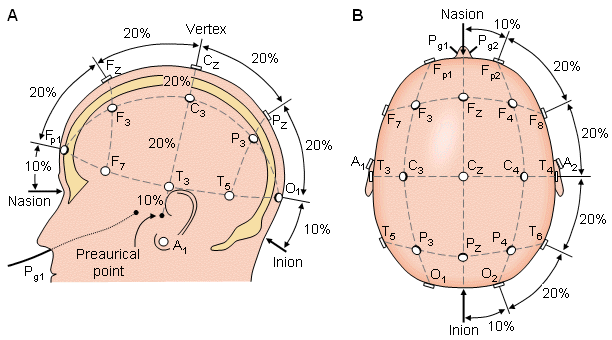
\includegraphics[scale=0.5,width=1\textwidth, inner]{EEG-10-20-Electrode-Placement}
%\caption{EEG 10-20 Electrode Placement System}
%\label{fig:figure1}
%\end{figure}
%
%Based on the picture above, What does each electrode's name stand for? Explain the naming method used in the 10-20 EEG system.
%\newpage
%
%\subsection{Alzheimer's Disease}
%Alzheimer's Disease (AD) is a progressive and irreversible neurological disorder that affects the brain, primarily causing problems with memory, thinking, and behavior. It is the most common cause of dementia, a general term for a decline in cognitive ability severe enough to interfere with daily life. \par
%The exact cause of Alzheimer's disease is not yet fully understood, but it is believed to involve a combination of genetic, lifestyle, and environmental factors. The staging of the AD is associated with the accumulation of Amyloid- beta ($A\beta$) proteins in the brain. These depositions cause synaptic and neuronal loss, which leads to major cognitive dysfunction in the advanced levels of the disease.\par
%
%While EEG is not currently used as a primary treatment for Alzheimer's disease, it can be a valuable tool in the diagnosis and monitoring of the disease. EEG can help in the diagnosis of Alzheimer's by detecting abnormal patterns of brain activity that are characteristic of the disease. In individuals with AD, EEG often shows changes such as a reduction in certain brainwave frequencies and an increase in others. These patterns can aid in differentiating Alzheimer's from other types of dementia or cognitive disorders.
%
%\subsection{Frequency Bands of EEG}
%In the frequency domain, EEG signals are divided into 5 bands.\cite{freq-bands}
%
%
%\begin{figure}[H]
%    \centering
%    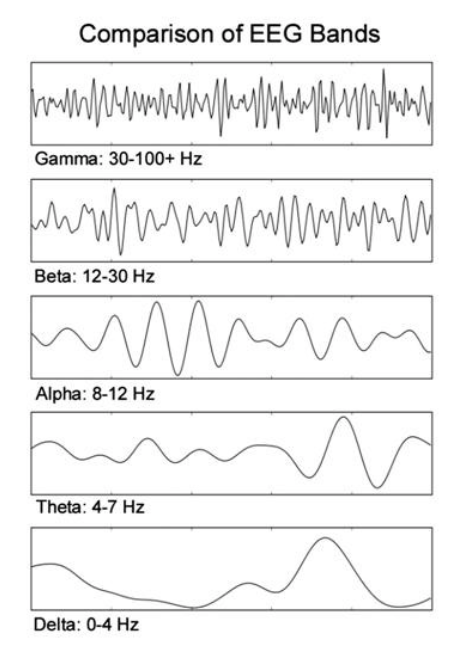
\includegraphics[scale=0.5]{freq-bands} 
%    \caption{EEG Frequency Bands}
%    \label{ffig:figure2}
%\end{figure}
%
%
%\par 
%Determine the activities each frequency band is associated with.
%
%\subsection{Sampling frequency}
%Based on frequency bands and Nyquist criterion, which sampling frequencies are preferred for EEG signals?
%\newpage
%
%% ------------------Section 3--------------------
%\section{EEG Signal Processing}
%In this section, firstly you would get familiar with the task and the structure of the data. 
%
%\subsection{Task Definition}
%\label{sec:sec3.1}
%\cite{EEG-Dataset}
%To identify the effect of olfactory dysfunction among different brain health states, the following task was performed to collect the data. The same sequence of stimuli was presented to all participants. The stimulation sequence was composed of two different odors, one occurring frequently (standard) with a probability of 0.75 and the other presented rarely (deviant) with a probability of 0.25. Each trial consisted of a 2s stimulus presentation followed by 8s of rest (pure water vapor). The odors were delivered to the participants using a laboratory olfactometer. The experiment involved 120 trials in which 90 frequent and 30 rare stimulation cycles were presented in a predetermined, randomized order. Lemon essence was used as the frequent odorant and rose essence was used as the rare odorant. These odors were selected to avoid trigeminal system activation as the olfactory and trigeminal systems are interconnected and may interact with each other during exposure to certain stimuli \cite{olfactory-trigeminal}. The duration of odor presentation was set at 2s to enable regular breathing cycles for the participants.
%
%\subsection{Data Description}
%\label{sec:sec3.2}
%\cite{EEG-Dataset}
%The dataset consists of three files as follows:
%
%\begin{itemize}
%    \item \texttt{AD.mat}: Contains data for Alzheimer’s disease patients.
%    \item \texttt{Normal.mat}: Contains data for healthy elderly participants.
%    \item \texttt{MCI.mat}: Contains data for mild cognitive impairment patients. (Described in part \hyperref[sec:5.1]{5.1})
%\end{itemize}
%
%The structure of the files is the same. Each file is organized as a structure array, in which each row contains information of one participant and the three columns correspond to the “epoch”, “odor” and “noisy” fields as described in Table 1.
%
%
%\begin{table}[]
%\begin{center}
%    \begin{tabular}{  | l | p{13cm} |}
%    \hline
%    Field & Description  \\
%    \hline
%    epoch & This is a 3D array structured as 4 × 600 × Num\_trials. The first dimension indicates EEG channels respectively from the first column as Fp1, Fz, Cz, and Pz. The second dimension contains EEG samples from 1 s pre stimulus to 2 s post stimulus, which at a 200 Hz sampling rate amounts to 600 samples. The last dimension shows the number of trials. This could be different for each participant as some trials were deleted during preprocessing. \\
%    \hline
%    odor  & This is a 2D binary array shaped as Num\_trial × 1. This array shows the odorant type (lemon/rose) the participant was exposed to in each trial. The value = 1 indicates the rose odor and the value = 0 indicates the lemon odor. \\
%    \hline
%    noisy & This is a 2D array with the size 1 × Num\_noisy. This array indicates noisy trials identified based on comparing the instantaneous and average trial amplitudes. These noisy trails can be ignored in processing and were included for the dataset completeness.\\
%\hline
%    \end{tabular}
%    \label{tab:table1}
%\end{center}
%\caption{Description of each structure array (.mat file) in the dataset.}
%\label{table:Data-Structure}
%
%
%\end{table}
%\newpage
%
%
%\subsection{Pre-Processing}
%Using a standard pipeline in EEG signal preprocessing is crucial for ensuring consistency, reproducibility, and objectivity in research. It reduces bias, enhances the reliability of results, and provides established best practices for addressing common challenges. A popular and widely used pipeline for EEG signal preprocessing is Makoto's pipeline (\href{https://sccn.ucsd.edu/wiki/Makoto's_preprocessing_pipeline}{\texttt{Makoto’s preprocessing pipeline - SCCN}}).\\ 
%
%The collected raw data from all participants were preprocessed following the full pipeline of Makoto with the use of EEGLAB and posted as a dataset, as described in the following steps:
%
%\begin{enumerate}
%    \item  Apply 1 Hz high pass filter to remove baseline drifts.
%    \item  Apply relevant notch filter to remove the 50 Hz line noise.
%    \item  Reject bad channels as a critical step before average referencing with the use of \texttt{clean\_rawdata()} EEGLAB plugin.
%    \item  Interpolate the removed channels.
%    \item  Re-reference the data to the average of all channels to obtain a good estimate of referenceindependent potentials.
%    \item  Apply \texttt{clean\_rawdata()} for cleaning the data by running artifact subspace reconstruction(ASR).
%     \item  Re-reference the data to the average again to compensate for any potential changes in the data caused by the previous step.
%    \item  Run independent component analysis (ICA) to identify EEG sources as well as the sources associated with noise and artifacts.
%    \item  Fit single and bilateral (if available) current dipoles.
%    \item  Further clean the data by source (dipole) selection using \texttt {IClabel()} plugin in EEGLAB.
%\end{enumerate}
%
%In the \texttt{Dataset/Preprocess} folder you can find the raw data for 2 subjects with the corresponding additional information provided. In this section you are required to preprocess these data and save your final preprocessed cleaned data.\\
%However, there is no need to fully implement the Makoto's pipeline and a simplified version of this is as follows; follow the instructions below and provide the required results in each step:\\
%    \begin{figure}[h]
%        \center 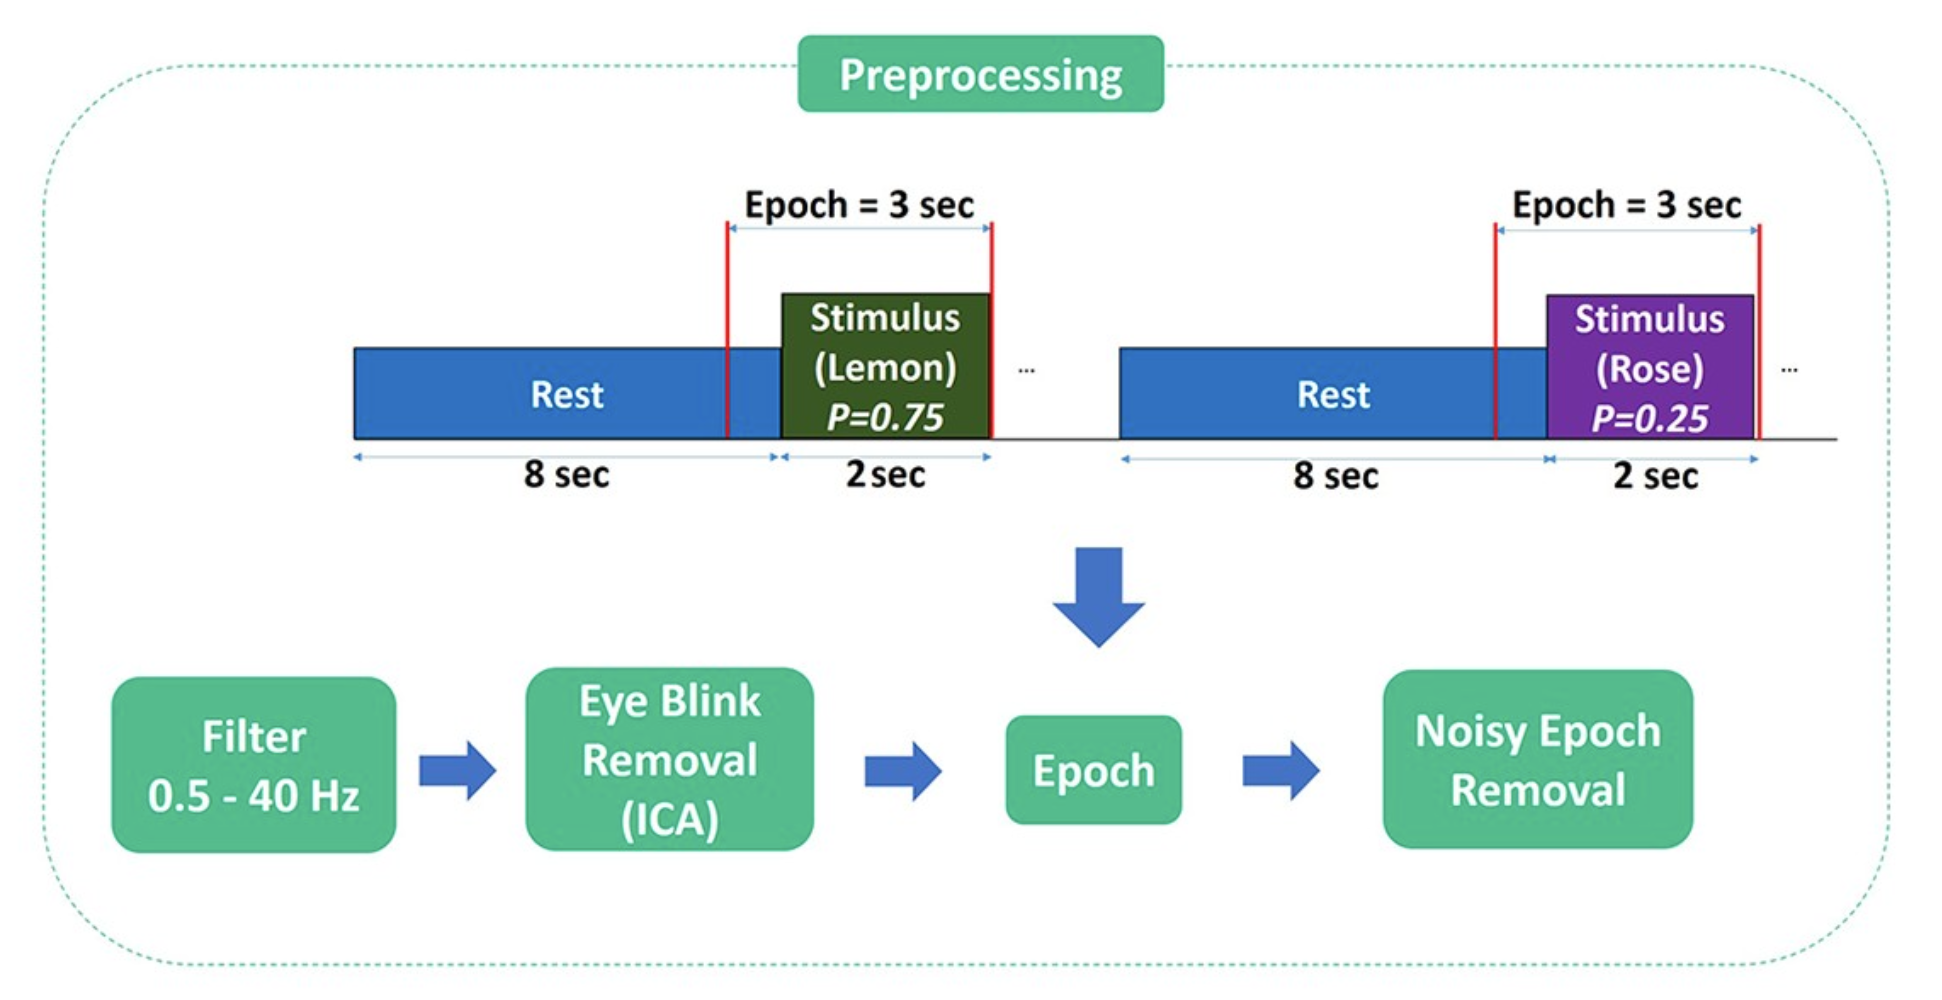
\includegraphics[scale=1,width=0.8\textwidth]{Images/Preprocess.png}
%        \caption{Task and Preprocessing Steps \cite{olfactory-deficit-AD}}
%        \label{fig:fig3}
%    \end{figure}
%\begin{itemize}
%    \item \textbf{Step 1}: To preproccess using EEGLAB, first re-reference data to the mean of the channels. Then use a bandpass filter to filter 0.5 - 40.5 Hz frequencies. As we have filtered to 40.5 Hz, there is no need to apply a 49.9 - 50.1 Hz notch filter to remove the line noise (However, keep this step in mind as this is a crucial step in EEG signal preprocessing!). Using FFT function or EEGLAB, plot the frequency spectrum of \texttt{Fz} channel data. (Just to note, your data will be saved at EEG struct in MATLAB workspace.)\\
%    
%    \item \textbf{Step 2}: In this part you would remove the artifacts of the signal. Artifacts include blinking, eye movement, muscle movement, heart rate and etc. For this, load your data at EEGLAB. Now load \texttt{Standard-10-20-Cap19.loc} file from \texttt{edit-channel loacations} menu that contains locations of channels. Then run ICA (Independent Component Analysis) algorithm from \texttt{tools-decompose data} by ICA menu. Please note that this part would probably takes more time. Then you will have the a figure like \hyperref[fig:fig4]{Figure 4} by running \texttt{tools $\rightarrow$ classify components using ICLabel-label components.}
%    \begin{figure}[h]
%        \center 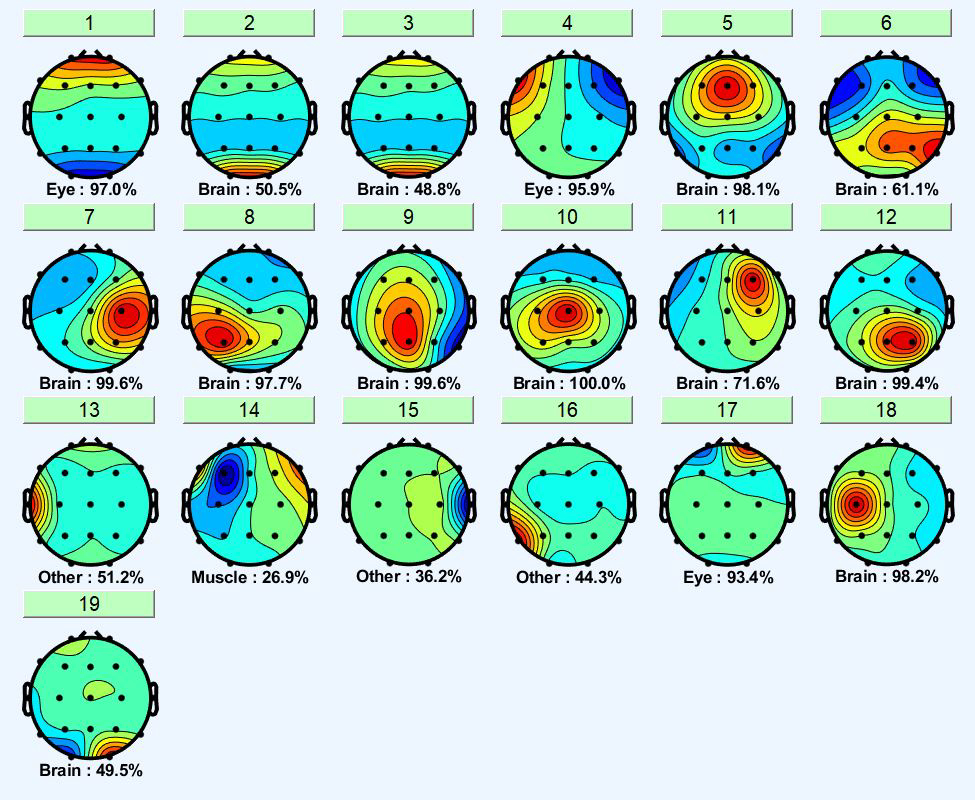
\includegraphics[scale=1,width=0.6\textwidth]{Images/brain_map.jpg}
%        \caption{An example of ICA components}
%        \label{fig:fig4}
%    \end{figure}
%    By clicking on each component, you can some details about it as well. Present a figure from one of the brain components with its details. \par
%    Now remove all non-brain components. For this purpose, from \texttt{Tools-remove components from data} enter the number of components that must be removed. \\
%    
%    \item \textbf{Step 3}:  Epoch the data of each subject. Epoch is a 3D matrix of the shape \{\texttt{Num\_Channels $\times$ Samples $\times$ Num\_Trials}\}. In fact, all data must be reshaped as the following figure suggests:
%    \begin{figure}[h]
%        \center 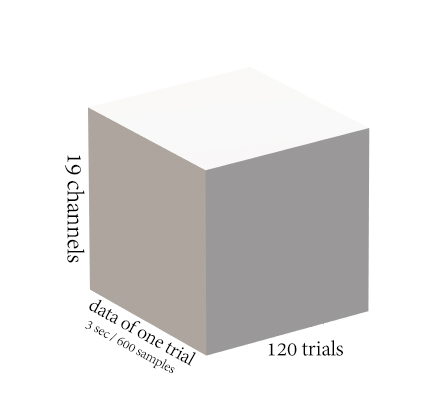
\includegraphics[scale=1,width=0.4\textwidth]{Images/epoch.jpg}
%        \caption{Epoch}
%        \label{fig:fig5}
%    \end{figure}\\
%    For epoching the data, starting point of the experiment is required. This is provided in the \texttt{help} file for each subject. Please note that you must epoch the data by considering this time as the start. Also, the data after 120 trials should be neglected as well.
%    
%    \item \textbf{Step 4}: In this step, you need to remove noisy trials. There are two ways to achieve this:
%    \begin{enumerate}
%        \item Observe data at EEGLAB and remove any trial that seems noisy. (\textsc{Preferred!})
%        \item Using power spectrum of each trial, remove trials that their standard deviation of their power spectrum is bigger than 3.5 .Create a 3D matrix by each trial's power spectrum for each channel using \texttt{pspectrum} in MATLAB. You can use the following commands to find noisy trials:
%        \begin{lstlisting}[style=Matlab-editor]
%vr = sum(nanstd(p,[],2).^2,2);
%noisy_trials = find(abs(zscore(vr))>3.5);
%        \end{lstlisting}
%        
%        In these commands, \texttt{p} is a matrix of frequency spectrums of all trials of a channel. \texttt{noisy\_trials} contains the number of noisy trials of that channel. These commands must run for each channel individually and the resultant noisy trials must be accumulated over all channel. Then remove all \texttt{noisy\_trials} from your epoch.
%    \end{enumerate}
%
%    \item \textbf{Step 5}: In the final step, only subsample the data corresponding to the \texttt{Fp1, Fz, Cz \& Pz} channels. You can find the channels' orders in the \texttt{Channels.jpg}.
%\end{itemize}
%
%Do these 5 steps for each subject and save the final data through an \texttt{struct} with the same format as described in \hyperref[tab:table1]{Table 1}. Also, consider the order of \texttt{odor} being the same as the ones used for normal participants.
%
%
%
%    
%\newpage
%
%\subsection{Phase Locking Value (PLV)}
%\label{sec:3.4}
%    Phase Locking Value (PLV) is a metric used to quantify the degree of phase synchronization or phase consistency between two oscillatory signals. It assesses the relationship between the phases of two signals at a specific frequency range. PLV is commonly used in the analysis of neural signals, including electroencephalography (EEG) and magnetoencephalography (MEG), to investigate the synchronization of oscillatory activity between different brain regions or across different frequency bands within a single region.. It provides insights into the functional connectivity and coordination of neural activity. \par
%
%    \medskip
%    PLV ranges from 0 to 1, where a value of 1 indicates perfect phase synchronization, while a value close to 0 represents a lack of synchronization. High PLV values suggest that the phases of the two signals are consistently aligned or coupled, indicating strong synchronization. This synchronization can reflect functional interactions between brain regions or coordinated activity within a network. In contrast, low PLV values indicate weaker or desynchronized activity, suggesting less functional coupling between the signals.\par
%
%    \begin{itemize}
%        \item What does phase synchronization indicate from a functional point of view? Discuss its importance with valid references. \medskip
%        
%        \item Formulate the definition of PLV and briefly discuss the mathematical tools needed to calculate it. \medskip
%
%        \item Implement a function which finds the PLV between two channels in a specific frequency range. This function is going to be needed in the \hyperref[sec:sec4]{section 4}. (\textsc{Note}: You are allowed to define this function with any required input arguments.)   \end{itemize}
%\newpage
%
%% ------------------Section 4--------------------
%\section{Results}
%\label{sec:sec4}
%In this section, you need to present the required results to assess the difference of Phase Locking Values (PLV) among two groups, namely AD and Normal in the slow gamma frequency range, which is 35 to 40 Hz.\par \medskip
%To fairly compare your results in this part, you do not need to use your preprocessing data from section \hyperref[sec:sec3.3]{3.3} and the preprocessed data of 15 healthy (normal) (age = 69.27±6.65, female = 53.33\%) individuals and 13 AD patients (age = 75.31±9.90, female = 61.54\%) are availabe through \texttt{Dataset/Normal.mat} and \texttt{Dataset/AD.mat}.\\
%
%
%    \subsection{Values} Find the PLV for all participants of both groups on both frequent and rare odors between the \texttt{Fz} and \texttt{Cz} channels using the function you implemented in section \hyperref[sec:3.4]{3.4} . \medskip
%    
%    \subsection{Distributions} Draw the box plots of PLVs you found in the previous part among two groups and two odors. Also, fit a gaussian distribution on these PLVs and present you results. You need to specify the corresponding \texttt{p-values} to evaluate the statistical significance of your findings. \medskip
%    
%    \subsection{Statistical Significance} Based on the \texttt{p-values} you founded in the previous part, discuss whether we could state that the "PLV is significantly different among AD and Normal subjects in the slow gamma frequency range". \medskip
%
%    \subsection{Phase Difference} Draw a polar histogram of the phase difference between \texttt{Fz} and \texttt{Cz} channels during frequent odor trials for a random subject in each group and compare the results. Also, plot the mean value of this quantity among all the subjects of each group and discuss the results.
%
%    \subsection{Heatmaps} Now you need to plot a heatmap which has the PLVs between each pair of the channels. Find whether PLV between other channel pairs are significantly different among two groups in the slow gamma frequency range and test your results. (\textsc{Note:} You need to provide \texttt{p-values} for your hypothesis if you found any significantly different channel pairs apart from (\texttt{Fz},\texttt{Cz}).)
%
%\newpage
%
%% ------------------Section 5--------------------
%\section{$^*$Bonus}
%\subsection{Mild Cognitive Impairment (MCI)}
%\label{sec:5.1}
%Mild Cognitive Impairment (MCI) is the stage between the expected decline in memory and thinking that happens with age and the more serious decline of dementia. MCI may include problems with memory, language or judgment. People with MCI may be aware that their memory or mental function has slipped. \cite{mayo-MCI}
%\begin{figure}[h]
%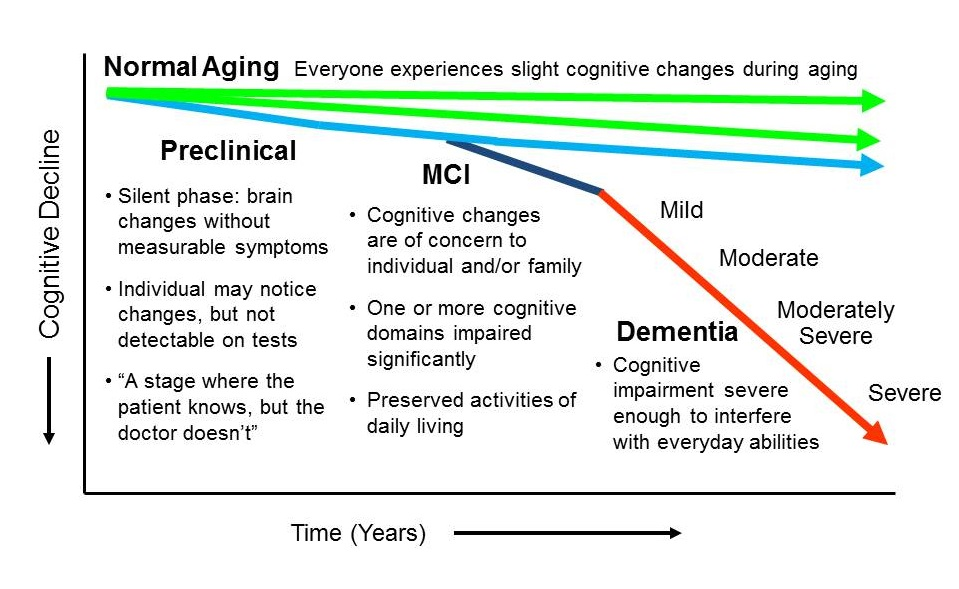
\includegraphics[scale=0.5,width=1\textwidth, inner]{Normal-aging-to-dementia.jpg}
%\caption{Normal Aging to Demantia Process}
%\label{fig:figure2}
%\end{figure}
%
%\subsubsection{Additional Information}
%Describe the relationship between MCI and AD. Explain whether MCI would always result in AD and briefly investigate the causes of MCI.
%
%\subsubsection{MCI Data Processing}
%In the provided dataset, you can find \texttt{MCI.mat} file. This dataset contains preprocessed cleaned EEG recording of the same task described in sections \hyperref[sec:sec3.1]{3.1} and \hyperref[sec:sec3.2]{3.2} for 7 MCI patients. \par
%Based on the significantly different coupled channels you found for differentiation between AD and Normal groups, find the Phase-Locking-Value (PLV) for the MCI subjects and provide the required results by comparing all the the 3 states (Normal, MCI, AD). Your findings must include the significance testing by providing the corresponding \texttt{p-values}.
%
%\subsection{Phase-Amplitude Coupling (PAC)}
%PLV was just one instance of the Phase-Amplitude Coupling (PAC) metrics. PAC is a form of cross-frequency coupling where the amplitude of a high frequency signal is modulated by the phase of low frequency oscillations. PAC is the most-studied type of cross-frequency coupling and is thought to be responsible for integration across populations of neurons. Low frequency brain activity controls the information exchange between brain regions by modulating the amplitude of the high frequency oscillations.\cite{PAC-nature}
%
%\subsubsection{Metrics}
%Conduct a search about other PAC measures and briefly provide an explanation about two of them.
%
%\subsubsection{Implementation}
%Implement one of the metrics mentioned earlier as a biomarker for distinguishing between AD and Normal groups. Present the relevant results through plots and provide a discussion regarding the efficacy of the selected metric.
%\\
%
%% ------------------Section 6--------------------
%\section{Conclusion}
%In this section, you are required to thoroughly examine and analyze the results you have obtained throughout this project. You must provide a comprehensive discussion of your findings, highlighting their significance and relevance to the research question. You should also present any limitations or weaknesses in your study and suggest possible areas for future research. Overall, this section is critical to demonstrating the quality and validity of your research and should be approached with careful attention to detail and clarity of expression.
\newpage
% ----------------------------------------------------------------------
% References
% ----------------------------------------------------------------------
\bibliographystyle{plain}
\bibliography{refs}

\end{document}